% !TeX root = ../thuthesis-example.tex

\chapter{基于树状区块链的跨链资产转移测试}

\section{实验说明}

现有的树状区块链以区域搜索区块链为基础,旨在解决车联网中节点过多,传统单链结构在面对大量节点时开销过大的问题。其设计按照Geohash编码的地理区域划分的具备区域地理位置状态特性的树状多链结构,根据Geohash编码的前缀匹配,表示父链与子链,形成了一个树状多链的结构。

应用到车联网当中,大部分车辆节点是树状结构的叶节点,用于维护区块链结构的节点不能随意改变其所属区域。但是车辆具有移动性,其不仅仅只是在其所属的区域内部活动,还存在从一个区域进入到另一个子链所管辖的区域的这种实际情况。此时,车辆账户进入到了新的一条子链当中,但是这条新的子链目前并不具备车辆账户的各种信息记录,且车辆账户在新链中资产为0,此时发送交易,便会因为账户余额不足而失败。为了能满足车辆账户的这种可移动性,在树状区块链中,当一个账户位置发生了跨子链(跨区域)的这种移动时,账户需要向一个管理账号发送一种特殊的交易,管理账户在接收到该交易时,将转移账户的资产余额从原先的子链中,转移到目标子链中,以此来实现账户跨子链时的资产的一致性。之后,账户便可以正常进行如发送交易等与区块链的交互操作。在树状区块链中,同一个账户同时只允许在一条子链中有资产余额,此时该链便被称为该账户的活跃链。

需要注意的是,不同于传统区块链的跨链资产转移,传统区块链的跨链资产转移大部分是为了实现不同区块链上资产的交换,其本质是针对不同记账体系之间资产转移过程,此时,或者整个转移过程依赖于可信的第三方,如跨链桥、跨链协议,或者需要对区块链进行结构上的扩展,如实现侧链。本节提出的跨链资产转移也可以理解为是跨区域的资产转移,是整个树状结构中的子链之间的资产的相互转移。

本节要进行的实验测试,便是针对树状区块链的这一跨链转账功能的测试,主要测试目标为跨链转账功能的正确性及其性能表现。

\section{结合源码分析实验}

关于跨链资产转移的代码实现主要在eth/handler.go中的handleMsg函数中,在这个函数中,实现了检索并解码传播新的区块时需要进行的操作。若想进行跨链资产转移,只有当前区块是分支区块,在接收到了叶子区块的请求时才会进入跨链资产转移的判断。此时,该交易信息需要提交含有txtype属性值的一个变量,若其为1,则此时分支节点在验证后将新的交易添加到pending列表中,记录\verb|Tx_request|的请求;若其为2,则此时分支节点会根据发送方的地址和输出链将\verb|Tx_out|与相应的\verb|Tx_request|进行匹配。若其为3,则此时分支节点根据收到的接收方的账户地址和输入链,将\verb|Tx_in|与相应的\verb|Tx_request & Tx_out|相匹配。同时,为了维护整个过程的原子性,分支节点会验证从转账请求开始的全过程(验证上一步交易的hash信息)。

\section{资产转移过程的事件介绍}

\begin{enumerate}
    \item 跨区域资产转移请求交易事件\verb|Tx_request|。首先,待转账账户在新进入一个子链后,此时,需要待转入账户主动向父链的资产管理账户(Asset Management Account,下简称AMA)发起跨区域资产转移请求交易sendTransaction,交易内容为 (from : account, to : AMA, txtype:1)。
    \item 资产转出交易事件\verb|Tx_out|。账户来源链需要向父链的资产管理账户发出资产转出交易,交易内容为 (from : account, to : AMA, value : balance(account), txtype:2, hashed : hash(\verb|Tx_request|)),这里需要上传前一步交易事件的hash值,用于分支节点的验证。
    \item 资产转入交易事件\verb|Tx_in|。在上一步验证成功之后,在新的目标链中,由资产管理账户向该账户发送资产转入交易,交易内容为 (from : AMA, to : account, value : balance(account), txtype:3, hashed : hash(\verb|Tx_out|))。同样上传前一步交易事件的hash值,用于分支节点的验证。
    \item 资产转移状态记录事件\verb|Tx_result|。若成功完成上述资产转移过程,则此时,在来源链中,由资产管理账户向该账户发送交易记录,交易内容为 (from : AMA, to : account, txtype:3, hashed: hash(\verb|Tx_in|))
\end{enumerate}

注意,资产转移交易被设定为特殊的交易类型,不消耗GAS,同时也并不考虑位置信息。

\section{设计资产转移实验}

在分析完底层的源码实现后,便可以据此来设计资产转移交易的实验测试脚本。目标:设计并进行数组跨链转账测试,验证转账测试的可行性,同时测试其性能表现。

为测试跨链转账实验,现构建如图\ref{fig:车辆与乘客跨链移动}的场景,模拟车辆与乘客账户的跨链移动时所进行的跨链的资产转移。

\begin{figure}
	\centering
	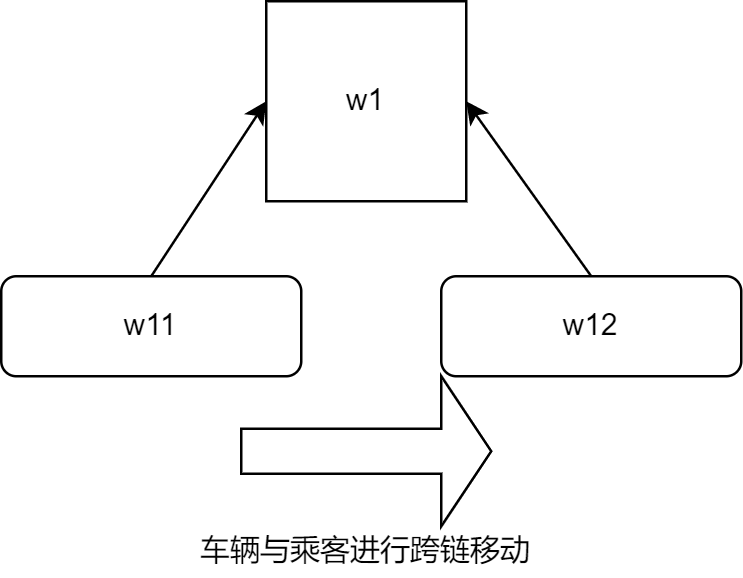
\includegraphics[width=0.5\textwidth]{figures/车辆与乘客跨链移动.png}
	\caption{车辆与乘客跨链移动}
	\label{fig:车辆与乘客跨链移动}
\end{figure}

构建一条主链记为w1,其下有两条子链分别记为w11和w12,表示的实际意义是,w1管辖Geohash编码前缀为w1的区域,w11和w12分别管辖Geohash编码前缀为w11的区域和w12的区域。此时,构建对应的区块链网络之后,在w11、w12的两条链中初始化相同的账户,各包含三个预分配账户以及10个普通账户,实验设计对于w11链中的普通账户,初始均分配有10000单位的初始资产,w12链中的普通账户,则初始资产均为0;希望模拟在账户位置进行从w11到w12的移动时,所进行的资产转移实验。具体操作为,开始实验后,树状区块链串行遍历w11中的普通账户,并发起上述的4个转账事件,将其资产转入w12链中。记录整个转账过程开始和结束的时间戳。

待试验完成之后,检查两条链中账户的资产情况便可验证,跨链转账实验的可行性,同时根据输出的时间戳来分析其性能表现。

\section{具体实验步骤}

具体的实验代码以及实验操作说明文档已存入我的毕设仓库,本小节只是简单说明一下大致流程。

\begin{enumerate}
    \item 构建上述的树状区块链网络结构,按照实验操作说明文档执行相应脚本文件即可。
    \item 依次启动两个子链开始挖矿。
    \item 由于本次实验要测试多个账户的跨链转账,且上述的转账事件有着严格的先后顺序,因此,为维护转账事件的次序性,另启动一个终端,运行branchnode-remastered.js脚本。该脚本监视父链w1的输出日志,并根据日志信息,向区块链发送交易事件,可以很好的维护转账事件的次序性。
    \item 运行脚本\verb|node transfer_test_step1.js|向w11链中的普通账户添加10000的初始金额,等待脚本运行完毕,验证w11链上的账户金额,可以发现初始金额设定成功
    \item 确认金额后,运行脚本\verb|node transfer_test_step2.js|,此时便开始了转账实验,终端中也不断发出各种转账事件的输出信息,等待转账事件全部发送完毕后,停止挖矿,实验完毕。
    \item 此时验证w11与w12中账户的资产信息。
    \item 执行\verb|node query_transfer_time.js|,脚本将访问链 w11 和链 w12 上
    的所有区块,统计其中包含的交易及其详细信息,生成测试结果报告。
\end{enumerate}

\section{测试结果分析 }

\subsection{实验正确性}

实验结果显示,原链w11中各账户的余额均为0,而链w12中的对应账户余额为10000 单位,证明了跨子链转账功能的正确性。

\subsection{性能展示}

本小节测试了10个账户的自身跨子链资产转移的测试,并分别记录了账户的转账耗时,从账户发起转账请求时开始记录,到账户资金转入目标链后结束。实验结果如图\ref{fig:账户跨子链资产转移所消耗的时间}所示:

\begin{figure}
	\centering
	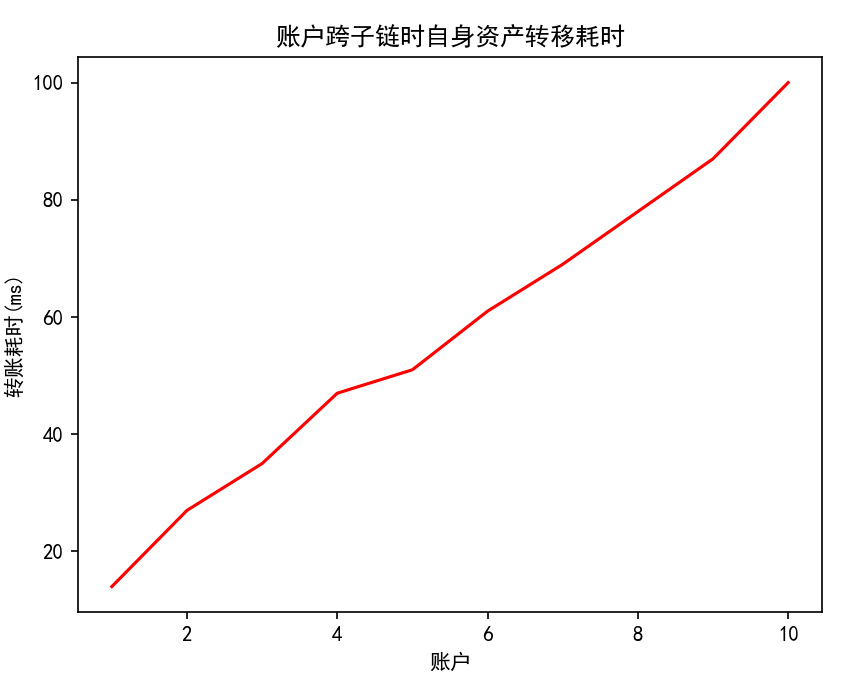
\includegraphics[width=0.8\textwidth]{figures/账户跨子链资产转移所消耗的时间.png}
	\caption{账户跨子链资产转移所消耗的时间}
	\label{fig:账户跨子链资产转移所消耗的时间}
\end{figure}

根据实验结果可以看出,账户所消耗的时间与账户的数目大致呈线性正相关。产生此现象的原因其实也并不难理解,从原理实现的角度来看,树状区块链的分支区块在处理跨链资产转移请求时,需要串行的处理并验证转账过程中相互通信的交易信息,由于跨链资产转移操作的通信过程所发送的交易信息有着严格的先后顺序,因此整个过程对外可以大致认为是一个原子性操作,耗时与账户数目线性正相关。

\section{本章小结}

本章主要介绍了树状区块链的跨链的资产转移功能。首先,阐述了实验的设计思路;之后,结合源码分析了其具体的实现过程,本章还介绍了跨链资产转移的过程中的事件函数。基于此,本章设计了账户的跨链资产转移实验,并经实验得出结论,账户跨子链进行资产转移所消耗的时间与账户的数目之间的关系大致呈线性正相关。

